% \documentclass[10pt]{scrartcl}
\documentclass[10pt,twocolumn]{scrartcl}

\usepackage[utf8]{inputenc}
\usepackage[T1]{fontenc}
\usepackage[ngerman]{babel}

\usepackage{amsmath}
\usepackage{amssymb}

\usepackage{graphicx}
\usepackage{tabularx}

\setlength{\parindent}{0cm}
\setlength{\parskip}{3mm}
\setlength{\textheight}{23.8cm}
\setlength{\headheight}{1cm}
\setlength{\topmargin}{-10mm}

\setlength{\oddsidemargin}{0cm}
\setlength{\evensidemargin}{0cm}
\setlength{\textwidth}{16cm}
\setlength{\columnsep}{8mm}

\usepackage{multicol}
\usepackage{colortbl}
\usepackage{xcolor}
\definecolor{grau}{gray}{0.95}
\definecolor{dunkelgrau}{gray}{0.85}

\usepackage[normal]{caption}
\usepackage{lipsum}

\setlength{\parindent}{5mm}
\setlength{\parskip}{0mm}

\usepackage{float}
\restylefloat{figure}

\renewcommand{\topfraction}{0.75}
\renewcommand{\textfraction}{0.2}

%###########################################################
% die Sachen mit der Kopfzeile
\usepackage{lastpage}
\usepackage{fancyhdr}
\fancyhf{} % leere alle Felder
\fancyhead[R]{\footnotesize Dr. Holger Gerhards \\ Kontakt: holger.gerhards@web.de}
\fancyhead[L]{\footnotesize Ausgewählte Methoden der
Datenanalyse, \\ Modellierung und Simulation} % Titel des Aufsatzes
\fancyfoot[C]{\footnotesize \thepage/\pageref{LastPage}}
% \fancyfoot[C]{\footnotesize \thepage}
\renewcommand{\headrulewidth}{0.4pt} % obere Trennlinie
\pagestyle{fancy}
%###########################################################

\newcommand{\ownsection}[1]{\begin{center}\LARGE\bf#1\end{center}}

\begin{document}

\twocolumn[
\ownsection{Ausbreitung von Infektionskrankheiten innerhalb einer Population}

\begin{center}
Marvin Klose (Marvin.Klose@sap.com) \\
Mannheim, November 2014
\end{center}
\vspace*{5mm}
]

% \begin{multicols}{2}

\section*{Abstract}
Jährlich sterben Millionen von Menschen an den verschiedensten Krankheiten. Sie infizieren dabei sich durch Übertragungswege wie Tröpfchen, Kontakt, Lebensmittel oder Trinkwasser. Medikamente und Therapien gibt es für fast alle bekannten Krankheiten, dennoch gibt ist Krankheiten mit tödlichem Ausgang. Deshalb ist interessant zu beobachten, wie sich Krankheiten unter bestimmten Parametern ausbreiten und wie Faktoren wie Resistenzen den Verlauf verändern können. Um schon möglichst präventiv Maßnahmen treffen zu können, damit erst gar keine Pandemie ausbricht und die Zahl möglicher Todesopfer zu minimieren. Der aktuellste Fall einer solchen akuten Bedrohung ist Ebola, welches momentan noch hauptsächlich in Westafrika auftritt. Dieses Themengebiet is nicht nur in der Biologie relevant, sondern lässt auch auf die Informatik übertragen. Computer können sich über Netzwerke und das Internet ebenfalls mit solche Viren oder Würmern anstecken. Dies ist jedoch nicht Bestand der Ausarbeitung.

\section*{Einleitung}

Die hier vorgestellte Ausarbeitung entstand im Rahmen der Vorlesung \glqq Ausgewählte Methoden der Datenanalyse, Modellierung und Simulation\grqq\; an der Dualen Hochschule Baden-Württemberg.
In der Vorlesung wurde ein Modell entwickelt, mit dem Ziel die Ausbreitung von Infektionskrankheiten zu simulieren.
Zentrale Aspekte sind deshalb die Gesundheit der Bevölkerung und die Veränderungen der Bevölkerungszahl, aufgrund von Epidemien. Somit lässt sich das Thema wissenschaftlich unter dem Begriff der Epidemiologie einordnen.
Dass das Thema nach wie vor Relevanz hat, sieht man an der aktuellen Ebola Epidemie, die sich hauptsächlich in Afrika ausbreitet. Zudem haben auch schon in der Vergangenheit immer wieder Epidemien Aufsehen erregt. Darunter beispielsweise 2006 die Vogelgrippe  \cite{gehlhoff2007chronik}
oder 2000/2001 BSE \cite{Spon:2014}. Diese forderten jedoch im Vergleich zur spanischen Grippe, die mehrere Millionen Menschen das Leben kostete, vergleichsweise wenig Todesopfer. Die spanische Grippe war die bisher verheerendste Influenzapandemie und forderte etwa 50 Millionen Todesopfer \cite{welt:2014}. Zusätzlich spricht man bei HIV/AIDS ebenfalls von einer Pandemie bei der nach Angaben der Organisation UNAIDS seit Bekanntwerden der Krankheit zwischen 35 und 43 Millionen Menschen gestorben sind  \cite{UNAIDS:2014}.
Damit ist ein Ziel des Modells die bestmöglichen Gegenmaßnahmen zu treffen, um die Bevölkerung zu schützen und so die Anzahl der Todesopfer zu minimieren.
Das vorgestellte Modell simuliert dazu die Entwicklung verschiedener Krankheiten innerhalb einer Population über einen gewissen Zeitraum. 
\smallskip

Inhaltlich beginnen wir mit der Erläuterung bestehender Modelle der Wissenschaft. Anschließend folgt die Vorstellung des von uns entwickelten Modells, das wir im Anschluss daran mit SIR-Modell vergleichen wollen. Darauf folgen die Ergebnisse und eine Diskussion. Abschließend gibt es einen Ausblick, der mögliche Erweiterungen unseres Modells behandelt. 


\subsection{Modelle in der Wissenschaft}
Ein Ansatz zur mathematischen Betrachtung der Krankheitsausbreitung ist das SIR-Modell von William O. Kernack und Anderson Gray McKendrick.\\
Es ist 1927 mit dem Zweck die Verbreitung Krankheiten sowie den Folgen von Gegenmaßnahmen von gesundheitsbezogenen Zuständen und Ereignissen in Bevölkerungen oder Populationen zu untersuchen.\\
In diesem Abschnitt wird zunächst die Idee hinter dem SIR-Modell vorgestellt, dann die Mathematik hinter dem SIR-Modells erklärt und abschließend aufbauend darauf die Frage beantwortet, warum gerade dieses Modell für den Vergleich des Projektes mit bekannten Methoden aus der Wissenschaft gewählt wurde.
\subparagraph{Theorie des SIR-Modells}
\begin{figure}
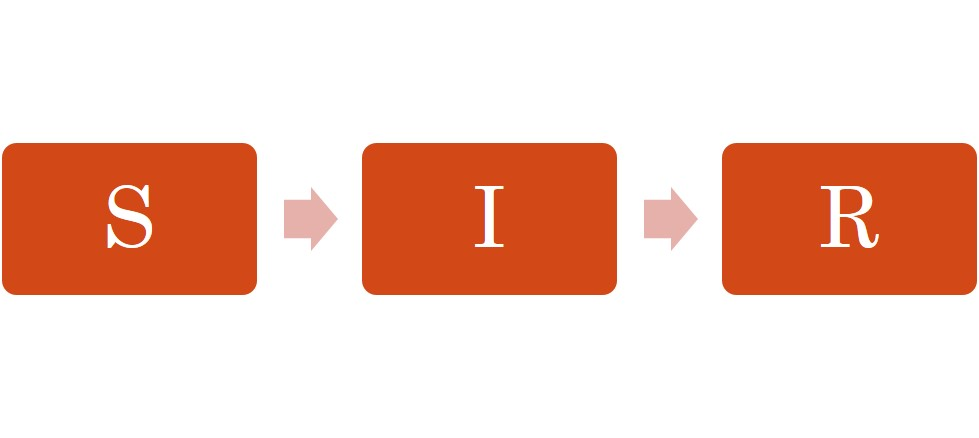
\includegraphics[width= 0.3\textwidth]{./images/SIR-Modell.jpg}\caption{Zustandsmodell des SIR-Modells}\label{fig:SIR}
\end{figure}
Das SIR-Modell ist eine mathematische Herangehensweise, bei der der Krankheitsverlauf statisch über feste Funktionsterme errechnet wird. \\
Dazu wird eine geschlossene Gruppe \textbf{N} an Individuen betrachtet. Die Anzahl \textbf{N} ist die Gesamtgröße der Bevölkerung. Die Bevölkerung setzt sich aus gesunden, kranken und \glqq R\grqq-Individuen zusammen, sodass gilt:
\begin{equation}\label{eq:N}
N = S + I + R
\end{equation}
Das heißt, die Bevölkerung wird in drei Zuständen klassifiziert:
\begin{itemize}
\item \textbf{S (Susceptible)} Anfällige Individuen, die innerhalb der Bevölkerung Infiziert werden können.
\item \textbf{I (Infected)} Infizierte Individuen, die Anfällige anstecken  oder in den \glqq R\grqq -Zustand übergehen können.
\item \textbf{R (Recovered)} Individuen im \glqq R\grqq -Zustand. Ein infiziertes Individuum, was in den \glqq R\grqq -Zustand übergeht, bleibt im R-Zustand. Es gibt keinen Übergang aus dem \glqq R\grqq -Zustand zurück in einen der anderen Zustände. Der \glqq R\grqq -Zustand kann von daher Individuen beschreiben, die aus Epidemiologischer Sicht keinen Einfluss mehr auf den Rest der Gesellschaft haben. Dies könnten z.B. immunisierte, tote oder isolierte Personen sein.
\end{itemize}
Das Bild \ref{fig:SIR} zeigt das entsprechende Zustandsübergangsmodell zu den drei Bevölkerungsgruppen.\\
Zur Visualisierung des Krankheitsverlauf in einer Bevölkerung kann geeigneter Weise ein Koordinatensystem benutzt werden, dass die Anzahl der Individuen in Relation zur Zeit setzt.
Für jede Zustandsgruppe wird ein Graph in das Koordinatensystem gezeichnet, sodass ablesbar wie viele Individuen zu einem Zeitpunkt krank, gesund oder im \glqq R\grqq-Zustand sind.\\
Die Verteilung der Individuen in die jeweiligen Zustandsklassen ändert sich mit dem Fortschritt der Zeit \textbf{t}, ist die Krankheit nicht ausgestorben, die Infektionsrate oder \glqq R\grqq-Übergangsrate größer null und nicht alle Individuen im \glqq R\grqq-Zustand.
Für jeden Zeitschritt wird die Anzahl der Individuen in den Zustandsklassen neu berechnet.\\
Beispielsweise könnten nach einem Zeitschritt drei neue Individuen erkranken und ein Mensch stirbt. Damit nimmt die Gruppe  \textbf{S} um drei Individuen ab, die Gruppe \textbf{I} wächst entsprechend um drei und gibt gleichzeitig ein Individuum an die Gruppe \textbf{R} ab, sodass sich die Verteilung nach einem Zeitschritt wie in Bild \ref{fig:sch} ändert.
\subparagraph{Berechnung der Entwicklung mit dem SIR-Modell}
\begin{figure}
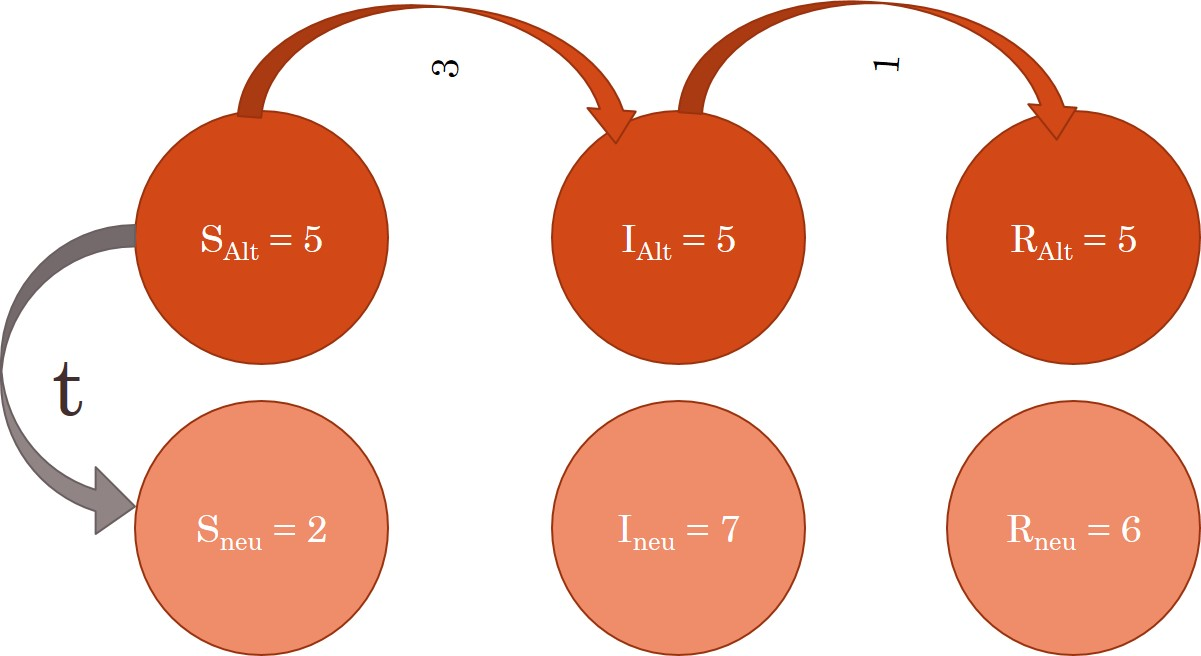
\includegraphics[width= 0.3\textwidth]{./images/SIR-Berechnung.jpg}\caption{Möglicher Zustandswechsel nach einem Zeitschritt}\label{fig:sch}
\end{figure}
Damit die Verteilung sinnvoll berechnet werden kann, werden Kennzahlen über die Krankheit benötigt, die das Krankheitsprofil widerspiegeln. Dabei wird für das SIR-Modell die Infektionsstärke und die \grqq R\glqq{}-Übergangsrate benötigt.
Über die Infektionsstärke $\lambda$ wird die Ansteckung-Kontakt-Rate \textbf{b} ermittelt \ref{eq:b}. Diese ist die Wahrscheinlichkeit mit der ein Individuum, dass mit \textbf{X} Individuen pro Zeitschritt Kontakt hat, erkranken kann.
\begin{equation} \label{eq:b}
b = ( \lambda * X ) / N
\end{equation}
Dabei ist die Anzahl X der Kontakte pro Zeiteinheit je nach Krankheitsübertragungsweg zu unterscheiden. Bei Krankheiten die über Tröpfcheninfektion übertragen werden, reicht Hände schütteln, die Übergabe von Geld oder sogar das Zusammensein in einem Raum zur Infektion. In diesem Szenario wird ein Durchschnittswert von 8 Menschen am Tag genommen.
Bei Krankheiten mit anderen Übertragungswegen z.B. AIDS muss der Austausch von Körperflüssigkeiten zur Infektion stattfinden, d.h. \textbf{X} zeigt den durchschnittlichen Austausch von Körperflüssigkeiten in einem Zeitabschnitt. In diesem Fall ist \textbf{X} im Durchschnitt natürlich deutlich geringer als bei Tröpfcheninfektion.\\
Über die Ansteckungs-Kontakt-Rate kann die Basisreproduktionsrate \ref{eq:R0} ermittelt werden. Diese beschreibt die Anzahl der Erwarteten Ansteckungen durch einen zusätzlichen Infizierten.
\begin{equation}\label{eq:R0}
R_0 = \frac{ b * N }{ \gamma }
\end{equation}
Hat man die beiden Größen ermittelt, können die Funktionen für die drei Zustände S, I und R über einen Zeitraum ermittelt werden. 
Es gilt:
\begin{equation}
\frac{ \delta S }{ \delta t } = -R_0 \cdot \frac{S * I}{N}
\end{equation}
Die erwartete Anzahl an Neuinfizierungen mal den Anteil der Gesunden und Infizierten Individuen von der Gesamtbevölkerung, ergibt die Anzahl der Gesunden, die diese Runde Infiziert werden. Die Menge der Anfälligen wird um die Menge der Neuinfizierten reduziert.
\begin{equation}
\frac{\delta I }{\delta t} = R_0 \cdot \frac{S \cdot I}{N}
\end{equation}
Diese Funktion berrechnet die Anzahl der Neuinfizierten von der Menge der Infizierten und der Anfälligen. Die Menge der Infizierten I wächst um die Menge der Anfälligen, die sich diese Runde infiziert haben.
\begin{equation}
\frac{\delta R }{\delta t} = \gamma \cdot I
\end{equation}
Die Anzahl der Individuen im R-Zustand wächst um einen Anteil $\gamma$ von den Infizierten. Das Heißt Einige Infizierte werden der Menge I abgeführt und wandern in Zustand R über. Von diesem Überstand ist kein anderer Zustand erreichbar, d.h. Diese Menge wächst stetig wenn $\gamma$ 0 und die Baisisreproduktionsrate größer null sind.

\subparagraph{Wahl des SIR-Modells als Referenzmodell}
\begin{figure}
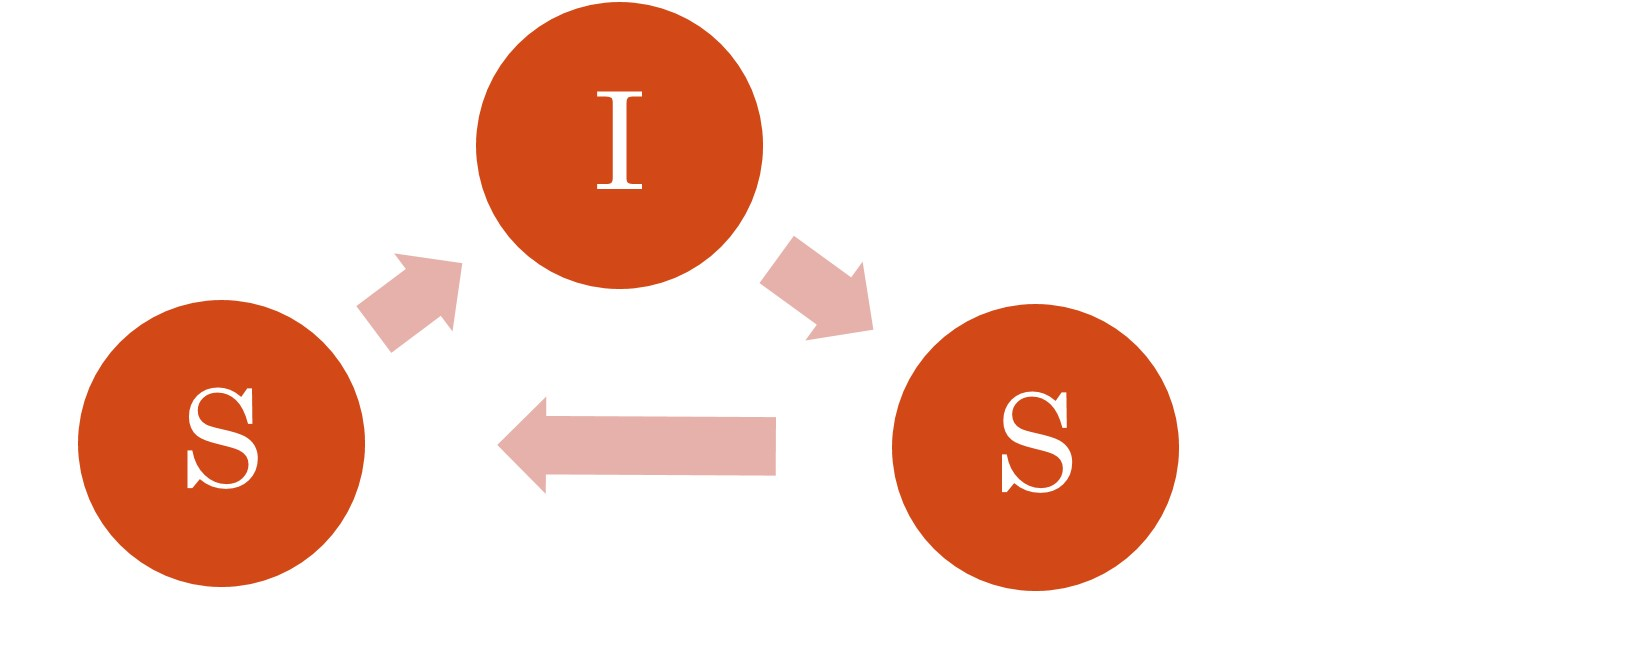
\includegraphics[width= 0.3\textwidth]{./images/SIS-Modell.jpg}\caption{Zuständsmodell des SIS-Modells}\label{fig:sis}
\end{figure}
Bei dem Vergleich mit bekannten Modellen aus der Wissenschaft drängt sich zunächst die Frage auf warum im Rahmen des Projektes gerade der Vergleich mit dem SIR-Modell angestellt wird und nicht mit einem anderen Modell zur Darstellung eines Krankheitsverlauf.\\
Wie genau ein mathematisches Modell die Krankheitsausbreitung in einer Gesellschaft beschreibt, hängt sehr davon ab, wie viel Realismus und damit wie viele Annahmen hineingesteckt werden.\\
Da in der Medizin viele Einflüsse zunächst vernachlässigt werden müssen, nicht bekannt sind oder die Krankheit sich mit der Zeit durch mutierende Viren verändert, haben die Modelle sehr selten einen endgültigen Charakter. Darüber hinaus sind Krankheiten in ihrer Entwicklung so unterschiedlich, dass es sehr oft möglich und manchmal nötig ist, die Modelle weiter zu verfeinern und anzupassen, wobei unterschiedliche Krankheiten unterschiedliche Modelle erfordern können. 
\cite{sebM}\\
Mit anderen Worten: Eine Krankheit kann mit all ihren Eigenschaften sehr realitätsnah abgebildet werden, aber möglicherweise bei einer anderen Krankheit schon wieder versagen. Von daher ist nicht das Modell, sondern das zugrunde liegende Szenario entscheidend für die Wahl des Vergleichsmodells. Eine sinnvolle Vorgehensweise ist es daher erst ein Szenario zu erschaffen und dieses dann mit einem geeigneten Modell abzubilden.\\ 
Im Rahmen unserer Projektes wurde sich für die Mittelalterpest entschieden.\\ 
Die Mittelalterpest war im 14. Jahrhundert gleichzusetzen mit einem Todesurteil. Beinahe jedes Individuum erlag nach einiger Zeit seiner Krankheit. Aus diesem Grund passt die Natur des Modells sehr gut zum vorgegebenen Szenario und dem Krankheitsprofil der Pest: Ein gesundes Individuum kann infiziert werden und dann sterben. In diesem Fall bildet der \glqq R\grqq-Zustand, die Anzahl der verstorbenen Individuen ab.\\
Mit einem anderen Szenario wäre es sinnvoll gewesen ein anderes Modell zu betrachten. 
Andere Modelle, die in der mathematischen Biologie angewendet werden sind z.B. das SI-Modell oder SIS-Modell.\\
Das Zustandsmodell im SIS-Modell ist im Gegensatz zum SIR-Modell zyklisch. Es gibt nur zwei Zustände: Anfällig und Infiziert. Anfällige Individuen können infiziert werden und dann wieder genesen und sich erneut infizieren, wie im Bild \ref{fig:sis}. Sind sie genesen können sie wiederum infiziert werden. Damit ist das SIS-Modell vor allem geeignet für bakterielle Erkrankungen wie z.B. Tuberkulose, bei der Individuen wieder genesen, aber keine Immunität entwickeln. \\
Das SI-Modell hat ebenfalls die beiden Zustände Anfällig und Infiziert, aber ist nicht zyklisch. Es können lediglich Individuen Infiziert werden. Diese bleiben endgültig im Zustand I.\\ 
Das SI-Modell ist also sinnvoll, wenn Individuen lediglich an einer Krankheit erkranken und nicht wieder genesen, aber auch nicht sterben. Das entsprechende Szenario, wäre also ein Virus, der ein Individuum auf Lebzeiten oder sogar darüber hinaus. Ein mögliches Szenario wäre ein aus Hollywood bekanntes Filmszenario der berühmten Zombie-Apokalypse.\\
Damit wird der erste Vorteil der Herangehensweise im Programm sichtbar: Während bei der mathematischen berechnen für jede Infektionskrankheit ein anderes Modell gewählt werden muss, um möglichst nah an der Realität zu bleiben, ist das Programm auf mehrere Szenarien mit Heilung, Toten, Resistenten etc. anwendbar.
\section*{Material und Methoden}
Zelluläre Automaten
Neuman Nachbarschaft...

\subsection*{Bedeutung der Abschnitte}

In naturwissenschaftlichen Veröffentlichungen sollte immer 
ein 'Abstract', eine 'Einleitung' und soetwas wie 'Ergebnisse und
Diskussion' vorhanden sein. Andererseits muss man sich bei den
Abschnitten wie 'Material und Methoden' und der 'Durchführung'
nicht zwingend an die Überschriften halten. 

Wichtig ist nur, dass man eingehens die Mittel, Techniken,
Methoden, vielleicht das mathematische Instrumentarium 
oder den experimentelle Aufbau erwähnt, mit welchem man 
gearbeitet hat und was essentiell zum Verständnis sein könnte.

Wenn Sie den Leser vorbereitet haben, was da kommt, dann können
Sie die große Synthese startet und ihr ganzes Setup mit allen
nötigen Parametern beschreiben, aus denen Sie letztendlich
die Ergebnisse generiert haben. Aus diesen Überlegungen heraus, 
sieht man bereits, dass die Grenzen zwischen den Bereichen 
'Material und Methoden' sowie 'Durchführung' und mitunter 
bis zu den 'Ergebnissen' verschwimmen können.

\subsection*{Ideen zum Lesen aus der Sicht eines Massenkonsumenten}

Da heutzutage enorm viele wissenschaftliche Artikel
eingereicht und veröffentlich werden, und das in zig verschiedenen
Journalen, kann niemand alles lesen und nur wenige haben die Zeit 
sehr viel zu lesen. Und da man als Leser noch andere Dinge im Leben 
vorhat, gibt es ein paar Techniken.
Diese Techniken spiegeln auch ein wenig die Bedeutung der einzelnen 
Abschnitte einer Veröffentlichung wieder.

Das Wichtigste ist natürlich die Überschrift, denn wenn diese außerhalb
der Interessensphäre des Lesers liegt, dann wird der Leser weiter suchen
und eine anderen Artikel heranziehen.

Danach wendet sich der Vielleser dem Abstract zu. Wenn dieses spannend ist,
wird dieser der Veröffentlichung mehr Zeit widmen. In Fächern wie der
Biochemie gibt es sogar Leute, die nur die Abstracts lesen, was durchaus
seine Berechtigung hat. Im diesen Abstracts stehen beispielsweise, 
wie bestimmte Proteine reagieren. Meistens ist das ausreichend für 
die eigene Forschung oder um etwas in Erfahrung zu bringen.
Übrigens sollte man im Internet theoretisch zu allen Veröffentlichung
die Abstracts mit dem Titel und den Autoren finden, die seit Anbeginn 
elektronischer Journals eingereicht wurden. Bei kostenpflichtigen 
Journals ist das Abstract wie der der Klappentext beim Buch und
entscheidet über Kauf oder Nichtkauf.

Die Diskussion könnte man als dritte Anlaufstelle nehmen. Wenn Sie 
die Ergebnisse, die im Abstract vielleicht bahnbrechend wirkten, genau 
beleuchtet wissen wollen, so sollten Sie hier mehr darüber
finden. Als Autor müßte man sich an dieser Stelle entsprechend 
kritisch mit den Ergebnissen auseinandersetzen. Auch ein Ausblick
ist manchmal sehr nett.

Als Viertes findet man noch eine hohe Informationsdichte in
Abbildungen, Diagrammen und Tabellen. Diese müssen so präsentiert werden,
dass man nicht hunderte von Zeilen Text durchforsten muss, damit man Sie versteht.
Dementsprechend braucht es eine Unterschrift bei Abbildungen und Diagrammen 
und einer Überschrift bei Tabellen wie es am Beispiel von Tab.~\ref{tab:falsch}
gezeigt wird. Achsenbeschriftungen, Einheitenangaben
und generell Übersichtlichkeit ist selbstredend zu beachten.
Andernfalls wird der Autor vielleicht als stümperhaft oder mindestens
wenig beflissentlich wahrgenommen.

\begin{table}[t]
\caption{Eine auffällig gefälschte Statistik über die Wissensaufnahme $\xi$
(in Wissenseinheit pro Minute) in Abhänigkeit von der verstrichenen Vorlesungszeit.}
\label{tab:falsch}
\centering
\begin{tabular}{cc}
\rowcolor{dunkelgrau}
Zeit [min] & $\xi$ [WE/min] \\
0 - 15 & 20 \\
\rowcolor{grau}
15 - 30 & 30 \\
30 - 45 & 42 \\
\rowcolor{grau}
45 - 60 & 70 \\
60 - 75 & 50 \\
\rowcolor{grau}
75 - 90 & 84
\end{tabular}
\end{table}

Wenn nun all das für den Leser interessant wirkte und dieser es vielleicht
selber im Detail nachvollziehen möchte, dann wird er sich wahrscheinlich
dem restlichen Text widmen.

Natürlich ist das eben Geschriebene nur eine Ideenskizze und wenn
Sie eine andere Herangehensweise an das Lesen solcher Artikel haben,
so steht dies Ihnen selbstverständlich frei.

\section*{Durchführung}
Wie bereits erläutert weißt das SIR-Modell einige Schwächen auf unter Anderem wird in dem Modell davon ausgegangen dass jeder Mensch im Schnitt acht Kontakte, je nach Modellierung, zu anderen Menschen hat. In unserem Programm wird dies dynamisch geregelt, dort gibt es einen Raster welcher einem Schachbrett ähnelt auf diesem beliebig großem rechteckigem \glqq{}Raster\grqq{} lassen sich an jeder $ x,y $ Position Zellen positionieren. So kann es Zellen geben welche sehr viele Nachbarn haben aber auch Zellen welche gar keinen Nachbar haben. Einen exemplarischen Raster sieht man in  Abbildung \ref{fig:Raster}. Auf diesem 3x3 Raster befinden sich aktuell drei Zellen theoretisch ist es aber auch möglich diesen Raster mit bis zu 9 Zellen zu besiedeln. So können auch extreme Situationen realistisch dargestellt werden wie zum Beispiel sehr dünn besiedelte Gegenden oder aber auch mittelalterliche Städte in denen in einem Haushalt durchaus 20 Personen lebten.\\

%Quelle recherchieren

\begin{figure}[t]
\centering
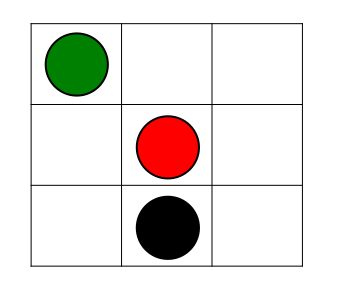
\includegraphics[width= 0.45\textwidth]{./images/nachbarn.png}
\caption{Ein 3x3 Raster mit Zellen in drei verschiedenen Zuständen}
\label{fig:Raster}
\end{figure}

\subsection*{Zelluläre Automaten}
Die vorliegende Implementierung basiert auf zellulären Automaten. Das heißt das jede Zelle erst einmal für sich unabhängig von anderen Zellen existiert.Eine Zelle ist im Kontext dieser Arbeit ein Mensch oder ein Tier. Dabei kann sich die Zelle in jeder Phase der Simulation nur in genau einem der folgenden Zustände befinden:
\begin{enumerate}
\item{\emph{Anfällig}\\
Eine anfällige Zelle kann nur von infizierten Zellen in ihrem direkten Umfeld welches durch eine Moore-Nachbarschaft \cite{Weisstein:2014} des Radius 1 charakterisiert wird angesteckt werden. Daraus folgt, dass eine Zelle auf dem rechteckigen Raster nur von den Zellen links über ihr, direkt über ihr, rechts über ihr, links und rechts neben ihr und links neben ihr, links unter ihr, direkt unter ihr und rechts unter ihr angesteckt werden kann.Dies sind im inneren des Spielfeldes maximal acht Zellen wie man am Beispiel der roten Zelle in Abbildung \ref{fig:Raster} gut sehen kann.\\
Des Weiteren wird auch betrachtet ob die Krankheit auch von jeder Zelle auf jede übertragbar ist oder ob zum Beispiel nur eine Übertragung von Mensch auf Tier aber nicht von Mensch auf Mensch möglich ist.\\
Angenommen die rote Zelle in Abbildung \ref{fig:Raster} ist ein infizierter Mensch und  die grüne Zelle ein gesundes Tier und die simulierte Krankheit lässt sich nicht von Mensch auf Tier übertragen. Demzufolge ist die grüne Zelle zu diesem Zeitpunkt vollkommen sicher, da sich in ihrer Nachbarschaft keine für sie potentiell gefährlichen Zellen befinden. 
}
\item{\emph{Infiziert}\\
Eine infizierte Zelle kann an ihrer Krankheit sterben, heilen und damit in den ersten Zustand übergehen, eine Resistenz bilden und damit in den dritten Zustand übergehen oder sie bleibt weiterhin infiziert.\\
All dies geschieht unter Berücksichtigung der für die simulierte Krankheit eingegebenen Werte.\\
Des Weiteren kann sie natürlich alle gesunden Zellen in ihrem Umfeld infizieren, auch dies geschieht unter Berücksichtigung der Werte die für die aktuelle Krankheit gelten.
}
\item{\emph{Resistent}\\
Da resistente Zellen nicht mehr in den Infiziert Zustand übergehen können und das Programm keine natürlichen Tode vorsieht, sind diese Zellen im Kontext des Programms unsterblich.\\
Sie werden jedoch trotzdem betrachtet, da sie im Kontext der Simulation interessant sind. So könnte man beispielsweise betrachten wie sich eine Krankheit verbreitet wenn bereits fast alle Zellen immun sind und es nur sehr wenige infizierte und anfällige Zellen gibt. Denkbar ist in diesem Szenario, dass die resistenten Zellen die infizierten Zellen weitestgehend abschirmen und so eine weitere Verbreitung verhindern. 
}

\item{\emph{Tot}\\
Eine Zelle in diesem Zustand, ist für die weitere Simulation nicht relevant. Naheliegenderweise kann sie sich nicht mehr eigenständig bewegen und auch kann sie keine anderen Zellen mehr infizieren. Es mag zwar durchaus Krankheiten geben welche auch nach dem Tot des Wirtes infektiös, an dieser Stelle wird in der Simulation davon ausgegangen dass die Zelle sich in einem intaktem Umfeld befindet in dem Tote entweder isoliert werden, dass sie keinen Kontakt mehr zu lebendigen Individuen haben. 
}
\end{enumerate}

\subsection*{Bewegung}
Zellen die sich in einem der ersten drei Zustände befinden können sich bewegen. Dabei wird in dieser Simulation davon ausgegangen dass die Zellen sich in einem geschlossenem Umfeld befinden. Es können also keine Zellen das Simulationsgebiert verlassen oder neu betreten.\\
Des Weiteren handelt es sich um eine zweidimensionale Simulation in der es nicht möglich ist dass sich mehrere Zellen auf einem Feld über- oder untereinander befinden.\\
Im allgemeinen Fall bewegen sich die Zellen dem Simple Isotropic  Random Walk Model \cite{Codling:2008} entsprechend, dies bedeutet dass sich eine Zelle zufällig in irgendeine Richtung bewegt unabhängig davon wohin sie sich zuvor bewegt hat. Dabei wird davon ausgegangen dass die Zellen grundsätzlich einen Drang zur Bewegung haben.\\
Sollte sich eine Zelle jedoch entscheiden sich in ein Feld zu bewegen indem schon eine andere Zelle ist, ist diese Bewegung nicht möglich und die Zelle muss sich neu entscheiden. Das Gleiche gilt für Zellen am Rand des Simulationsgebietes. Natürlich gibt es die Möglichkeit dass eine Zelle komplett \glqq umringt\grqq\; von anderen Zellen ist, in diesem Fall bleibt die Zelle zwangsweise an ihrer alten Position.\\
Veranschaulicht bedeutet dass das zum Beispiel die grüne Zelle in Abbildung \ref{fig:Raster} nur zwei Möglichkeiten hat sich zu bewegen. Nämlich eine Bewegung nach unten oder nach rechts. Da über und links neben ihr keine Felder mehr sind und auf der Diagonale kann sie sich auch nicht bewegen da dort die rote Zelle das einzig mögliche Feld blockiert.\\
%Quelle hier einbinden
\subsection*{Wirtsbeziehungen}
Die Simulation ist in der Lage einfache Wirtsbeziehungen zu simulieren, dadurch dass es zwei Arten von Zellen gibt (Menschen und Tiere), kann man krankheitsabhängig unterscheiden ob eine Krankheit jeweils von Mensch auf Mensch, von Mensch auf Tier, von Tier auf Mensch und von Tier auf Tier übertragbar ist, so kann schon eine beträchtliche Menge von Krankheiten simuliert werden.\\
Dies ermöglicht es zu simulieren was passiert wenn man versucht Krankheiten wie die Tollwut welche fast ausschließlich von Tieren auf den Mensch übertragen werden, versucht auszurotten indem man alle potentiellen Wirte immunisiert.

\subsection*{Bevölkerungsdichte}
Im Rahmen dieses Modell ist es möglich zu simulieren wie sich eine Krankheit bei verschiedener Bevölkerungsdichte verhält. So ist es möglich dass es auf einem gegebenem Raster $x\cdot y$ für die gilt $ x,y \in \mathbb{N}$ zwischen $1$ und $x\cdot y$ Zellen zu platzieren.\\
Dabei ist auch das Verhältnis von Menschen zu Tieren vollkommen beliebig wählbar. So lassen sich die Auswirkungen der Bevölkerungsdichte auf die Entwicklung simulieren.

\subsection*{Nicht deterministisch}
Ob eine Zelle in einen bestimmten Zustand übergeht hängt einerseits von ihrem eigenem Zustand und den Zuständen ihrer Nachbarn, andererseits von einer krankheitstypischen Wahrscheinlichkeit ab. Sollte eine Zelle infiziert sein und bei der simulierten Krankheit besteht die Wahrscheinlichkeit zu sterben bei 25\% so wird der Wert 0.25 mit einer zufälligen Zahl zwischen 0 und 1 verglichen. Sollte diese Zufallszahl größer sein als die Übergangswahrscheinlichkeit geht die Zelle in den entsprechenden Zustand über.\\
Das bedeutet das selbst wenn man die Simulation mit exakt den selben Parametern mehrmals durchführt man unterschiedliche Ergebnisse erzielen kann. Das Modell ist also nicht deterministisch.


%\begin{enumerate}
%\item{Bewegung}
%\item{\emph{Wirtsbeziehungen}
%
%
%
%}
%\item{\emph{Bevölkerungsdichte wird berücksichtigt}
%
%
%}
%\item{nicht deterministisch}
%\end{enumerate}

%Hier ein paar Regeln zum Schreiben eines Artikels, 
%gegen die ich teilweise in dieser Ausarbeitung bereits
%verstoßen habe.
%\begin{list}{-}{}
%\item[(a)] Schreiben Sie nicht in 'Ich'-Form! Versuchen Sie entweder 
%unpersönlich zu bleiben oder ggf. im Namen des Forschungsteams mit 'wir' zu arbeiten.
%
%\item[(b)] Sprechen Sie den Leser nicht an! Der Leser soll sich selber ein
%objektives Bild über den Artikel machen. Ich hoffe Sie verstehen das, oder?
%
%\item[(c)] Bilder, Diagramme und Tabellen stehen alleine. Im Text findet man
%nur die Referenzen darauf, wie Sie dies mit Bezug auf
%Abb.~\ref{fig:audio} ersehen.
%
%\item[(d)] Bilder, Diagramme und Tabellen sind nie vor der Seite der entsprechenden 
%Referenz im Text zu finden. Meistens findet man sie gesammelt im oberen
%Seitenbereich, der entsprechenden oder der nahen Folgeseiten. Die Positionierung
%im oberen Bereich der Seite hilft den Schnelldurchblätterer, dass seine 
%Augen nicht so viel springen müssen.
%
%\item[(e)] Gleichungen und Formeln wie beispielsweise das Faltungsintegral
%\begin{equation}
%g(t) = \int_{-\infty}^{+\infty}\!\!d\tau \; h(\tau) \, f(t-\tau)
%\label{eq:faltung}
%\end{equation}
%stehen niemals isoliert und sollen sich harmonisch in die Satzstruktur einfügen.
%Es empfiehlt sich bei neuen Variablen gleich unter der Gleichung, diese
%zu benennen bzw. zu erklären, damit der Leser nicht lange suchen muss.
%
%\item[(f)] Bezieht man sich auf eine Formel, weil man beispielsweise findet,
%dass die Integralschreibweise für die Korrelationsanalyse 
%\begin{equation}
%g(t) = \int_{-\infty}^{+\infty}\!\!d\tau \; h(\tau) \, f(t + \tau)
%\end{equation}
%dem Faltungsintegral aus Gl.~\eqref{eq:faltung} sehr ähnlich sieht,
%so sollte man anhand der hier getätigten Referenz die Umsetzung ersehen.
%
%\item[(g)] Zitieren Sie jemanden oder beziehen Sie sich nur auf eine
%Veröffentlichung wie beispielsweise auf ein interessantes Experiment 
%zur Totalreflektion \cite{Goos1947}, so können Sie dies beispielsweise 
%durch Nummern tun, die im Literaturverzeichnis ausgeführt sind.
%Andernorts findet man auch gern den Nachnamen des Erstautors und
%das Erscheinungsjahr als Schlüssel, um den Eintrag im Literaturverzeichnis
%zu finden. 
%
%Übrigens findet man in naturwissenschaftlichen Schriften 
%äußerst selten wörtliche Zitate und meist Referenzen, oder wollten Sie
%aus der Arbeit von Einstein zur Speziellen Relativitätstheorie \cite{Einstein1905}
%wörtlich zitieren?
%
%\item[(h)] Das Literaturverzeichnis sollte ausreichend Informationen enthalten,
%um die Veröffentlichungen auch zu finden. Ebenso muß es einheitlich für
%die einzelnen Veröffentlichungstypen wie Buch, Artikel, Webseite etc. sein,
%denn nur die Wenigsten mögen es, sich durch scheinbares Chaos fremder Leute zu wühlen.
%
%\item[(i)] Argumentieren Sie! Entschuldigen Sie sich nicht für Ihre Arbeit, 
%aber argumentieren und diskutieren Sie die Dinge, die merkwürdig sind.
%Führen Sie weitestgehend objektive Gründe an, wenn etwas nicht funktionierte.
%Argumentationen, Begründungen etc. müssen meist nicht lang sein, 
%aber über offensichtliche Wiedersprüche zu schweigen wirkt unprofessionell 
%und der verärgerte Leser wird vielleicht noch unliebsamere Worte 
%zum Lästern finden.
%
%\item[(j)] Vermeiden Sie Füllwörter! Obwohl man aber vielleicht auch behaupten
%könnte, dass dann auch ein wenig mehr Text gefüllt wird.
%\end{list}
%
%%\begin{figure}[t]
%%\centering
%%\includegraphics[width=0.45\textwidth]{Bilder/audio-signal-short.pdf}
%%\caption{Das akustische Signal von etwas Gestammelten, wobei die Amplituden in 
%%nicht näher zu bezeichnenden Einheiten (a.u. für arbitrary unit) angegeben sind.}
%%\label{fig:audio}
%%\end{figure}
\section*{Vergleich mit dem SIR Modell}
ZDF
\section*{Ergebnisse und Diskussion}
Vorteile
\begin{itemize}
\item Simuliert Bewegung
\item Wirtsbeziehungen
\item Szenarien möglich Grafische Darstellung
\item Dynamisches Modell

\end{itemize}
Nachteile
 \begin{itemize}
	\item Keine Inkubationszeit
\item Zelle besitzt kein Alter
\item Keine Geburtenrate
\item Reproduktion der Zellen
\item Resistente verschwinden nicht vom Raster
\item Nicht deterministisch
\end{itemize}




%Was Sie hier finden sollten, findet sich leider schon in den vorangegangenen
%Textpassagen und Abschnitten und ich mag Sie nicht mit Wiederholungen
%langweilen. Jedoch kann man ab und zu feststellen, dass das Abstract und
%die Diskussionen eine gewisse Ähnlichkeit aufweisen, wobei die Diskussion
%immer ausführlicher sein soll. Das liegt mitunter daran, dass beide 
%Abschnitte Zusammenfassungen mit unterschiedlicher Nuancierung darstellen. 
%
%Jetzt möchte ich mich gleich auf genau dieses Schreiben beziehen, 
%von dem ich hoffe, dass Sie hinsichtlich des Schreibens und Lesens 
%von solchen Ideen- und Gedankenmanifestationen etwas für sich mitnehmen konnten. 
%Selber hatte ich mit diesem Thema verstärkt während meiner Doktorarbeit \cite{Gerhards2008} 
%zu tun gehabt, ohne selber der enthusiastischste Leser gewesen zu sein.
%Viele Ideen und Ansichten habe ich jedoch von meinem Doktorvater 
%Prof. Dr. Kurt Roth mitbekommen, dessen arbeitsgruppeninterne Übungen 
%zum schnellen Lesen förderlich für die Adrenalinproduktion waren.

% Ziel der Vorlesung war neben der sehr theorielastigen Einführung
% in die Fourier-Transformation, Faltung, Korrelationsanalyse und
% der nichtlinearen Optimierung, dass Sie sich mit einem Problem
% mit stark physikalischem Schwerpunkt auseinandersetzen sollten.
% Hier galt es sich einzuarbeiten und danach die entsprechenden
% Werkzeuge zum Lösen des Problems sowie zur graphischen Visualisierung
% anzueignen. Die Päsentation sowie der Abschlussbericht stellen
% dann die mündliche, wie schriftliche Darlegung des Problems und
% dessen Lösunng dar.
% 
% Und auch wenn Sie mit Ihrem Problem in Zukunft nie wieder in
% Berührung kommen werden, ist es generell wichtig Probleme anzugehen,
% die Werkzeuge zur dessen Bewältigung anzueignen und danach die
% Problemlösung auch voranzutreiben. Wissenschaftlichkeit in den
% Sachverhalt einfließen zu lassen, bedeutet dann noch das Problem
% in einem größeren Kontext zu sehen oder auch in Bezug auf verwandte
% Problematiken.

% Zum Abschluss aber noch einen Witz: Stellen Sie sich eine Party
% vieler mathematischer Funktionen vor. Auf einmal öffnet sich die
% Tür und ein Differentialoperator tritt herein. Alle Funktionen
% suchen die Flucht, nur die e-Funktion bleibt an der Bar stehen.
% Kommt der Differentialoperator zur e-Funktion und fragt, warum
% sie denn nicht weglaufen täte. 'Na, ich bin doch die Funktion e hoch x.
% Du kannst mich nicht wegdifferenzieren.' Darauf antwortet der
% Differentialoperator: 'Aber ich leite doch nach y ab.'

%Schließen möchte ich mit einem Zitat von Wittgenstein \cite{Wittgenstein1922},
%welches Prof. Dr. Kurt Roth im Zusammenhang wissenschaftlichen
%Schreibens gerne nutzte: {\it Was sich überhaupt sagen lässt, lässt
%sich klar sagen; und wovon man nicht reden kann, darüber muss man
%schweigen.} 

\section*{Danksagung}
Brauchen wir nicht oder?
%
%Wenn es jemanden zu danken gibt, wie beispielsweise die Geldgeber, 
%dann ist hier der Ort. 
%
%Ich für meinen Teil möchte den Dank an Prof. Dr. Tobias Straub
%richten, für das Angebot eine Vorlesung an der Dualen Hochschule in
%Mannheim halten zu dürfen. Auch einen Dank an all die Studenten der Vorlesung
%und besonders für die spannenden Projekte, bei den ich teils auch 
%etwas hinzulernen durfte. Am Ende nochmals vielen Dank 
%an den bereits erwähnten Prof. Dr. Kurt Roth für alles, 
%was ich während meiner Doktorarbeit durch ihn gelernt habe.

\begin{thebibliography}{99}
\bibitem{Goos1947}F.Goos und H.Hänchen: {\it Ein neuer fundamentaler Versuch zur Totalreflektion}, 1947; Annalen der Physik 436, S. 333-346
\bibitem{Einstein1905}A.Einstein {\it Zur Elektrodynamik bewegter Körper}, 1905; Annalen der Physik und Chemie 17, S. 891-921
\bibitem{Gerhards2008}H.Gerhards: {\it Ground Penetrating Radar as a Quantative Tool with Applications in Soil Hydrology}, Heidelberg 2008; Dissertaton,
\bibitem{Wittgenstein1922}L.Wittgenstein: {\it Tractatus Logico-Philo\-so\-phi\-cus}, London 1922; Kegan Paul, Trench, Trubner \& Co., Ltd.
\end{thebibliography}

\end{document}